\documentclass[10pt]{article} 
\usepackage{amsmath, amsfonts, amsthm, amssymb, amscd, mathrsfs}
\usepackage{a4wide}
%\usepackage{lipsum}
\usepackage{authblk}
\usepackage{xcolor}  
\usepackage{graphicx,epstopdf,psfrag}
\usepackage{enumitem}
\usepackage[export]{adjustbox}
%\usepackage{fancyhdr}
\usepackage{color}

\newcommand \be {\begin{equation}}
\newcommand \ee {\end{equation}}
\newcommand\mat[1]{\ensuremath{\mathbf{#1}}}
\addtolength{\textwidth}{1cm}

\newcommand{\bt}[1]{\mathbf{#1}}
\newcommand{\todo}[1]{{\color{red} TODO: {#1}}}
%%%%%%%%%%%%%%%%%%%%%%%%%%%%%%
%\pagestyle{fancy}
\begin{document} 

\title{Adaptive Regression for the Lorenz Model}
\author[1,2]{Eugenia Kalnay}
\author[2]{An\i l Zengino\u{g}lu}
\affil[1]{Department of Atmospheric and Oceanic Science, University of Maryland, College Park, Maryland}
\affil[2]{Institute for Physical Science and Technology, University of Maryland, College Park, Maryland}
\renewcommand\Affilfont{\itshape\small}
\date{}

\maketitle

%%%%%%%%%%%%%%%%%%%%%%%%%%%%%%
\section{Introduction}
Model Output Statistics (MOS) is used to improve weather forecasts \cite{Glahn72, Carter89}. MOS is a linear regression method where the predictors are historical model forecasts (temperature, wind, etc.) and the predictands are observations at weather stations. MOS improves the accuracy of model forecasts by reducing the forecast bias and pushing the forecast towards climatology for long lead times. Much work goes into improving the quality and length of the training data set used to determine the regression coefficients. MOS typically requires extensive data collection to determine the regression parameters.

There are two difficulties with MOS of concern to us: (i) Models are updated frequently, which changes their bias and their associated regression parameters for MOS; (ii) Regression parameters are obtained through averaging over long observation intervals which loses information about weather-dependent seasonal and dynamic changes in bias.

Adaptive Regression (AR) may alleviate these problems. By taking into account only the recent weather, AR provides similar forecast improvements to MOS but allows for model upgrades and time-dependent bias correction. 

We report on a simple framework for performing Observing Systems Simulation Experiments (OSSEs) that compare MOS and AR forecasts under different circumstances for the Lorenz-96 model. 

\section{OSSE}

\subsection{The Lorenz-96 model}
The Lorenz-96 model is a chaotic, continuous-in-time, discrete-in-space, dynamical system that was proposed by Lorenz in 1996 as a toy model for weather dynamics \cite{Lorenz96}. It is a system of ordinary differential equations (ODEs) for variables $\{x_j\}$ with external forcing
\be \label{eq:model} \frac{dx_j}{dt} = ( x_{j+1} - x_{j-2} ) x_{j-1} - x_j + F(t). \ee
The variables may represent a meteorological observable observed at equidistant sites around a latitude circle \cite{LorenzEmanuel98}. The quadratic advective terms compete with the linear dissipative terms and the outcome of this competition as the asymptotic behavior of the solution is determined by the external forcing term. For small values of the forcing, linearity dominates and the solution is dissipative. For large values of the forcing, the nonlinearity dominates and the solution blows up. In an intermediate range of the forcing, the system behaves chaotically. This behavior makes the Lorenz-96 model a popular testbed for new ideas in atmospheric sciences \cite{LorenzEmanuel98,Boffetta02,Ott04,Pazo08, Karimi10, Majda17}. Remarkably, the chaotic behavior of the solution defined as the positivity of the top Lyapunov exponent has only recently been proven \cite{Bedrossian20}. 

\subsubsection{Simulation of the Lorenz model}

We integrate \eqref{eq:model} for $j=1,\dots,40$, using a 4th order Runge-Kutta scheme. The parameters are chosen following \cite{LorenzEmanuel98} as $F(t)=8$, $dt = 0.05$. Comparing the error growth timescale in \eqref{eq:model} with operational numerical weather prediction systems, one time step is considered in \cite{LorenzEmanuel98} to correspond to about 6 hrs. 

We choose random initial data from an approximately Gaussian distribution with mean $F/4$ and standard deviation $F/2$. To remove transient effects, we integrate the model forward for 90 days, that is, for $360$ time steps, and use the data at the last time step as initial data for our data assimilation experiments.

We refer to a 5-year evolution of the Lorenz system with constant forcing as {\it Nature}. Nature is the reference against which all forecasts are compared. 

\subsection{Forecasts}
Forecast accuracy in chaotic systems are limited not only by chaos (rapid divergence of nearby initial conditions), but also by the error in the underlying model \cite{Orrell01}. This model error is in general state-dependent. Statistical methods can be applied to mitigate the impact of model error on forecasts.

We introduce biases to the Lorenz-96 system by hand to simulate the impact of model error on forecasts. Each forecast is made with a biased model. The bias is modeled as a modification of the external forcing. We consider the following options
\begin{itemize}
\item Constant bias: 
\end{itemize}

In this work, we focus on forcing bias, random noise, and spatial bias which is a constant error term pushing the solution away from nature and depends on spatial location. While the observational error is an important source of error, it is not relevant to the current work and did not impact our results qualitatively.

A forecast is performed every day (every 4 time steps in the Lorenz system) starting from perfect initial data given by the nature run. The forecast length is 5 days. The forecast is made with a model that has a simulated and controlled source of error. We consider three models with bias and one model with noise. In Bias, we have a constant shift in the forcing term. In GridBias we add a random but constant vector to the solution. In TimeBias, we modify the forcing term in a time-dependent manner. In Noise, we add random noise to the solution during the time evolution.

\subsection{Model Output Statistics}
To focus on the differences between MOS and Adaptive Regression, we construct an Observing System Simulation Experiment (OSSE) where many of the surrounding technical difficulties encountered with real data are not present. In our OSSE, the nature run is given by the evolution of the Lorenz system \eqref{eq:model}. Observations are perfect and simply consist of the reading of the solution data. A model consists of a biased version of the Lorenz system. Forecasts have 5-day lead times and are produced with biased models. This setup allows us to demonstrate the interaction of various types of bias with statistical post-processing and construction of blended models. The regression coefficients are computed based on a 5 year training set (dependent data). The improvement of the MOS corrected forecasts is then measured on an independent 5 year run.

\subsubsection{Formalism}

We use simple linear regression where a single independent variable is used to predict the value of the dependent variable. The predictands $y^n=y(t_n)$ are obtained from a solution of the Lorenz system \eqref{eq:model}, and the predictors $x^n=x(t_n)$ are obtained from a solution of a biased Lorenz system.

Given the regression parameters $b_i$, the forecast equation based on linear regression reads
\[ \hat{y}^n = b_0 + b_1 x^n  \]
The coefficients $b_i$ are determined by minimizing the sum of squares of the forecast errors over the training period [Wilks 1995]
\[ SSE = \sum_{n=1}^N (y^n - \hat{y}^n)^2 = \sum_{n=1}^N (y^n - (b_0 + b_1 x^n))^2  \,.\]  
Solving $\partial (SSE) / \partial b_i = 0$ for the regression parameters we get
\be\label{eq:regr} \mathbf{b} = (\mathbf{X}^T \mathbf{X})^{-1} \mathbf{X}^T \mathbf{y}\,,  \ee
where 
\[ \mathbf{X} = 
\begin{pmatrix} 
1 & x^1 \\
1 & x^2 \\
\vdots & \vdots \\
1 & x^N 
\end{pmatrix}, \qquad 
\mathbf{b} = \begin{pmatrix} b_0 \\ b_1 \end{pmatrix}, \qquad 
\mathbf{y} =  \begin{pmatrix} y^1 \\ y^2 \\ \vdots \\ y^N \end{pmatrix}\,.  \]

Here, $\mathbf{X}$ is the dependent sample predictor matrix consisting of the model output variables, $\mathbf{b}$ is the vector of regression coefficients, and $\mathbf{y}$ is the vector of predictands in the dependent sample.

Plot dependent estimate of the error variance of the prediction! For independent data, the error variance is not that much larger. Show in plot.  We don't need cross-validation because we can simply produce a second set of 5 year data.


\subsection{Adaptive Kalman Regression}
In Adaptive Regression, we apply the Kalman Filter equations [Kalnay 2003] in a sequential formulation to the now time-dependent regression coefficients $\mathbf{b}^n = \mathbf{b}(t_n)$. The forecast at each time-step is made with time-dependent regression coefficients 
\[ \hat{y}^n = b_{0}^n + b_{1}^n x^n  \]
Kalman Filtering consists of two steps. In the first step, the coefficients $\mathbf{b}^n$ and their error covariance at time $t_n$ are forecast starting from the analysis at time $t_{n-1}$. In the second step, the Kalman weight is derived and the observations at time $t_n$ are used to obtain the analysis, which is more accurate than the forecast. In our case, the "forecast", or the first guess, is to keep the regression coefficients constant. The error covariance is as estimated in the previous time step, plus an additional error introduced by this "regression forecast model"
\begin{align}
\mathbf{b}_n^f &= \mathbf{b}_{n-1}^a,  \\
\mathbf{P}_n^f & = \mathbf{P}_{n-1}^a + \mathbf{Q}_{n-1}\,.
\end{align}
Here, $\mathbf{Q}$ is a diagonal matrix of tunable coefficients where we have assumed that the errors of the different coefficients are not correlated. The Kalman weight is given by
\[ \mathbf{K}_n = \mathbf{P}_n^f \mathbf{X}_n (\mathbf{X_n}^T \mathbf{P}_n^f \bt{X}_n + \bt{r}_n )^{-1}\,.\]
We update the regression coefficients by using the observations $y^o_n$ as follows:
\begin{align}
\bt{b}_n^a &= \bt{b}_n^f + \bt{K}_n (y_n^o - \bt{X}_n^T \bt{b}_n^f) \\
\bt{P}_n^a &=  (\bt{I} - \bt{K}_n \bt{X}_n^T) \bt{P}_n^f \,.
\end{align}
The tuning parameters are the observational error covariance $\bt{R}_n$ and the regression model error covariance $\bt{Q}_n$. 

\section{Comparison}

\subsection{Tests of MOS}
First we test the improvement provided by an optimal MOS setup. 

To construct nature, we start with random Gaussian initial data with mean $\mu=2$ and standard deviation $\sigma= 4$. The data is evolved for 90 days to remove transient effect and the last step is used as initial data for the nature run. nature is solved for 5 years and 5 days (the last 5 days are used to compare the forecast at the end of the 5 year period). The solution is evaluated at 4 stations that mimic weather stations at grid points $\{5, 15, 25, 35 \}$ (counting from 0). 

The forecasts with biased models are made daily starting from perfect initial data provided by the nature. We have experimented with observational error but noted that it did not affect our qualitative results.  

We test 3 different types of error in our models: forcing bias (fb) which consists of a positive deviation of the forcing term, $F$, from its actual value by 2; noise (ns), where a random Gaussian noise term is added at each time step with vanishing mean, a standard deviation of 0.02, and an amplitude of 2; grid bias (gb), where a random but constant bias term is added to all grid points with vanishing mean and a standard deviation of 4.  \todo{Implement time dependent forcing bias and add to this list.}

\begin{figure}[ht]
	\center
	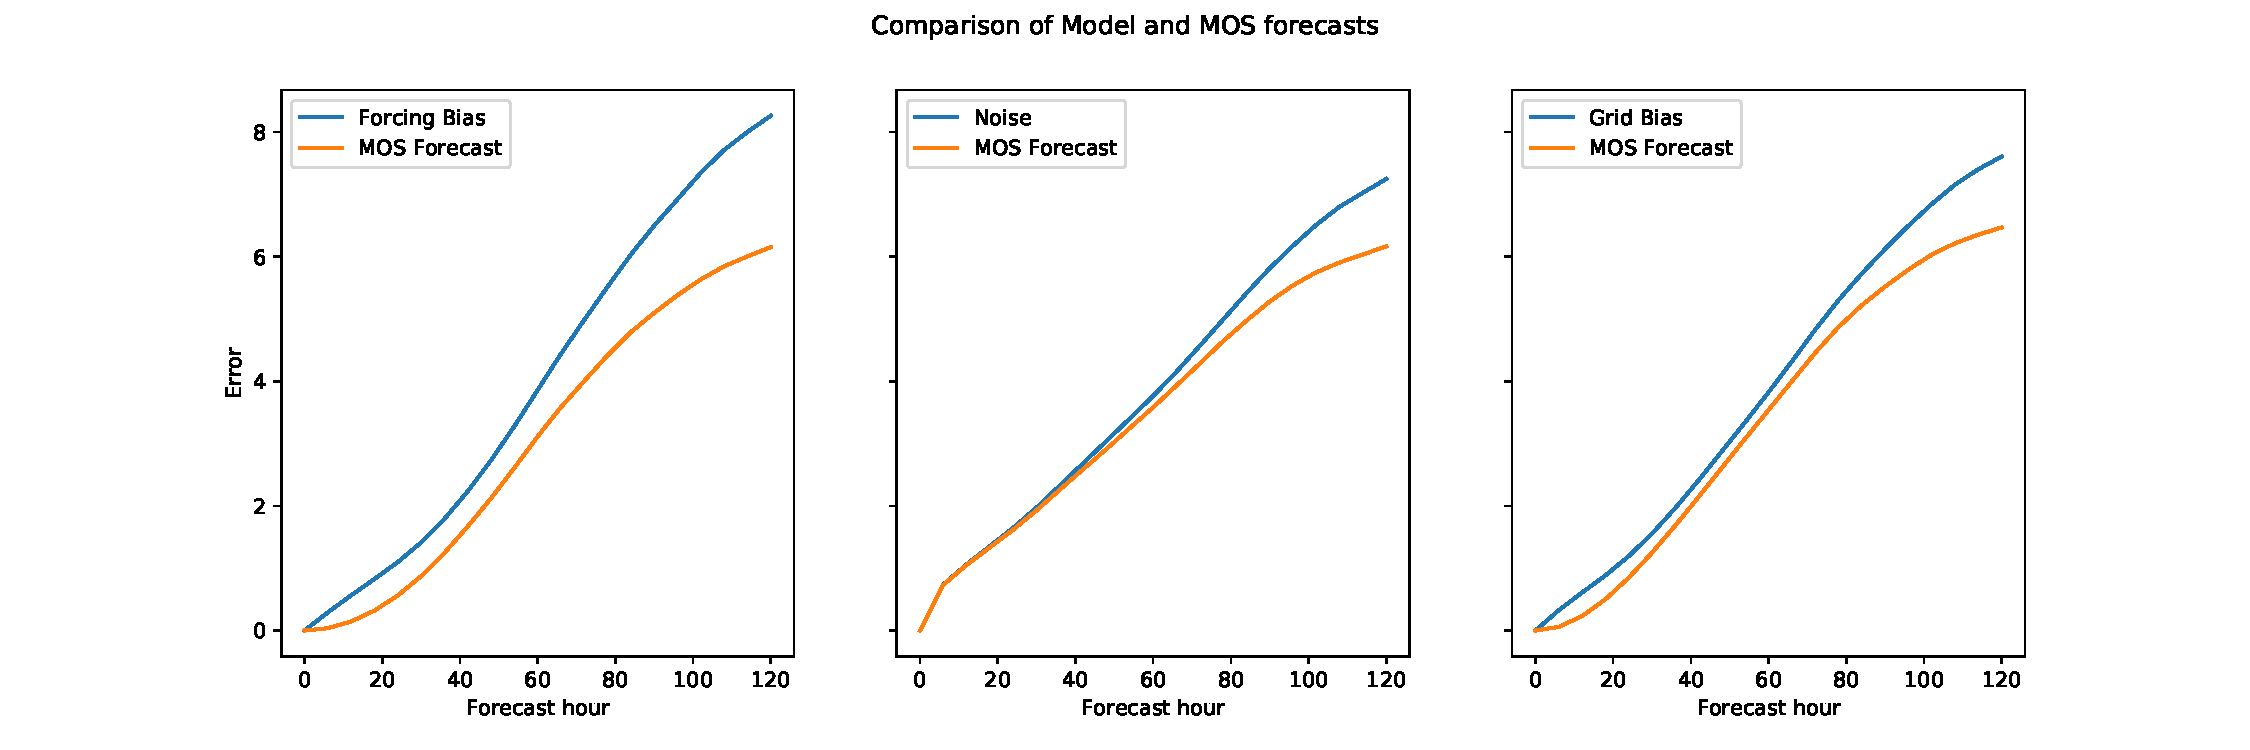
\includegraphics[width=\columnwidth]{figs/ModelMOS}
	\caption{For each model, the model forecasts have larger errors than the MOS-corrected forecasts. The difference is smallest for the noisy model, because bias correction does not improve noisy forecasts, except for long lead times where we approach climatology more efficiently with MOS-corrected forecasts.}
	\label{fig:MOS}
\end{figure}

We make daily forecasts with a lead time of 5-days with each model. A 5-year run is then used to determine the regression parameters at each of the 4 stations according to \eqref{eq:regr}. Next we create a new nature run and associated model forecasts. The MOS-corrected model forecasts are made using the regression parameters from the previous run. The difference between nature and forecast is plotted in Fig.~\ref{fig:MOS}. 


\begin{figure}[ht]
	\center
	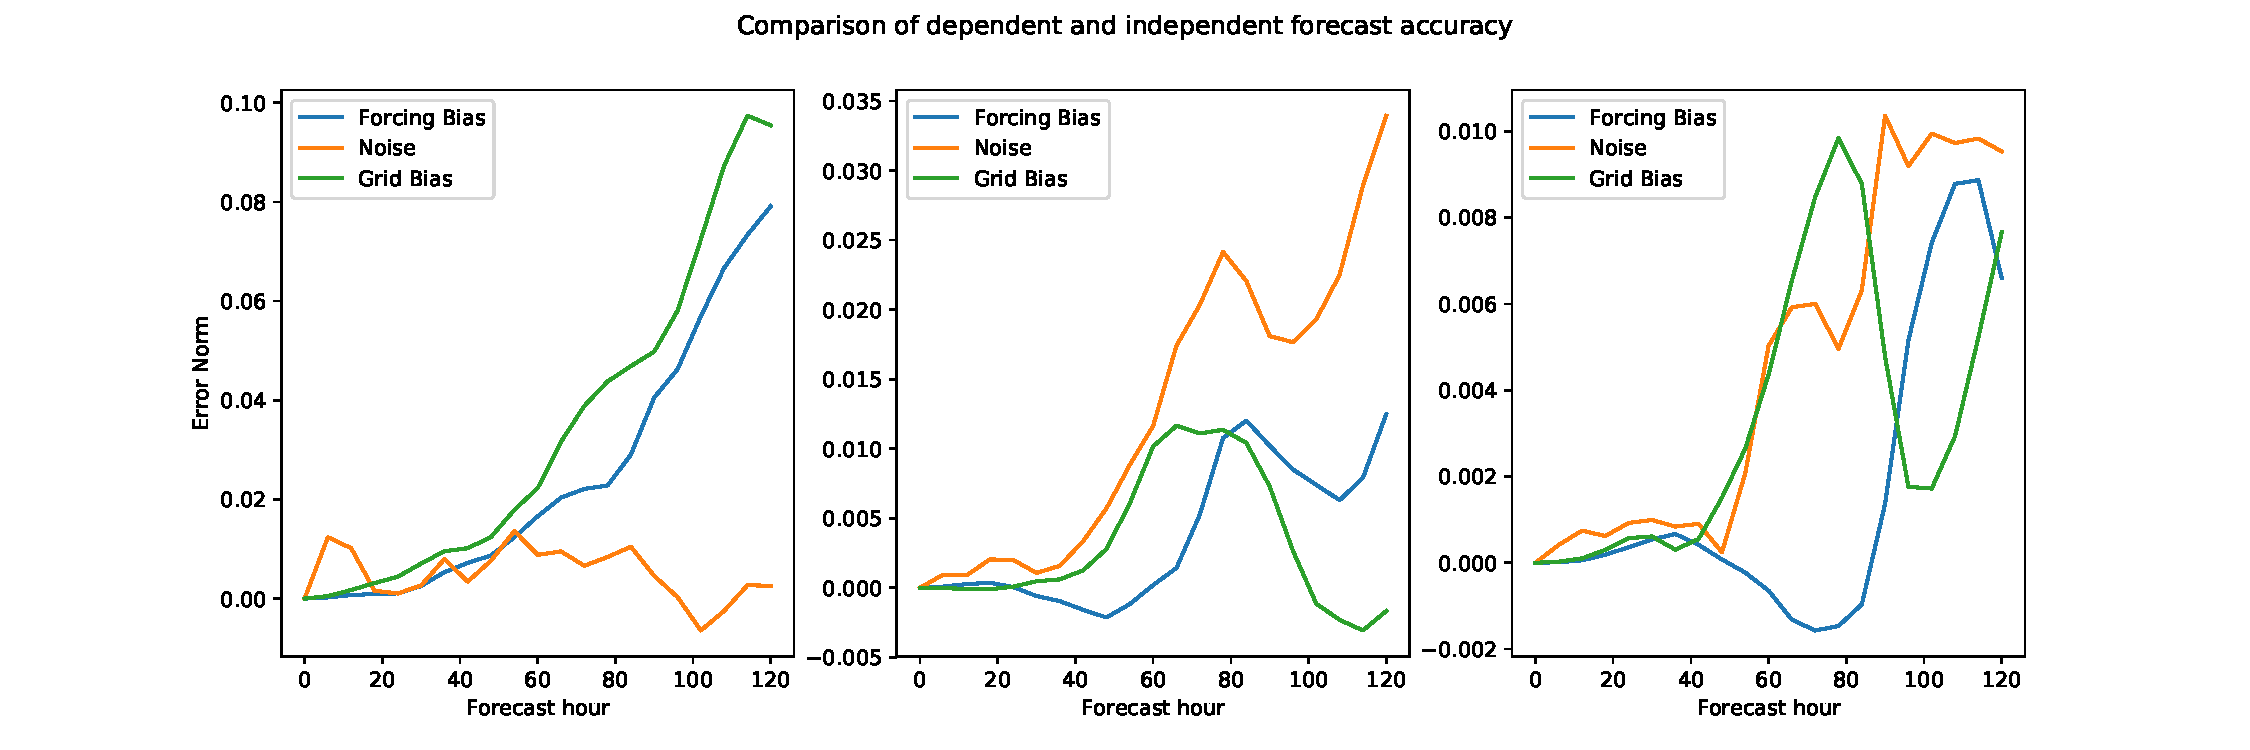
\includegraphics[width=\columnwidth]{figs/DepIndep}
	\caption{}
	\label{fig:indep}
\end{figure}


We found that the difference between dependent and independent are not large compared to the scale of Fig.~\ref{fig:MOS}. We expect the MOS forecasts to get better with the length of training data, which would imply that the difference between dependent and independent data would also be smaller for longer evolutions. As seen in Fig.~\ref{fig:indep} the difference between dependent and independent data is larger for shorter runs.  





\todo{GO ON HERE!}

The difference between dependent and independent data is on the order of $10^{-3}$ and is therefore not visible on the scale of the above figure. 



\subsection{Adaptive Regression vs MOS}

Our experiment is optimal for MOS in that the training period is long (5 years) and the model is unchanged both during the training period in the production of the dependent data and during the forecasts in the production of the independent data. Note that this is an unrealistic scenario. Operational models and data assimilation systems are frequently updated and do not satisfy these optimal criteria. The desire to be able to make frequent changes to the model are the dominant motivation behind the adaptive method tested in this paper.  




The biased models loose forecast skill at long lead times so the advantage of MOS forecast becomes more dominant as it asymptotes to the climatology error. 


\section{Discussion}



\appendix 
\section{Adaptive Regression Kalman Filter Algorithm}

The algorithm for adaptive regression using the Kalman Filter is as follows.
\begin{align*}
y_n^f &= \bt{X}_n^T \bt{b}_{n-1}^a, \\
\bt{P}_n^f &= \bt{P}_{n-1}^a + \bt{Q}_{n-1}, \\
e_n &= y_n^o - y_n^f, \\
\bt{K}_n &=  \bt{P}_n^f \bt{X}_n (\bt{X_n}^T \bt{P}_n^f \bt{X}_n + \bt{r}_n )^{-1}, \\
\bt{b}_n^a &= \bt{b}_{n-1}^a + \bt{K}_n e_n, \\
\bt{P}_n^a &= \bt{P}_n^f - \bt{K}_n \bt{X}_n^T \bt{P}_n^f\,.
\end{align*}



\begin{thebibliography}{99}

\bibitem{Glahn72} Glahn, H.R. and Lowry, D.A., 1972. The use of model output statistics (MOS) in objective weather forecasting. {\em Journal of Applied Meteorology and Climatology}, 11(8), pp.1203-1211.
\bibitem{Carter89} Carter, G.M., Dallavalle, J.P. and Glahn, H.R., 1989. Statistical forecasts based on the National Meteorological Center's numerical weather prediction system. Weather and Forecasting, 4(3), pp.401-412.
\bibitem{Lorenz96} Lorenz, E.N., 1996. Predictability: A problem partly solved. {\em ECMWF Proc. Seminar on predictability} (Vol. 1, No. 1).
\bibitem{LorenzEmanuel98} Lorenz, E.N. and Emanuel, K.A., 1998. Optimal Sites for Supplementary Weather Observations: Simulation with a Small Model, {\em J. Atmos. Sci.} 45, 399-414.
\bibitem{Boffetta02} Boffetta, G., Cencini, M., Falcioni, M. and Vulpiani, A., 2002. Predictability: a way to characterize complexity. {\em Physics Reports}, 356(6), pp.367-474.
\bibitem{Ott04} Ott, E., Hunt, B.R., Szunyogh, I., Zimin, A.V., Kostelich, E.J., Corazza, M., Kalnay, E., Patil, D.J. and Yorke, J.A., 2004. A local ensemble Kalman filter for atmospheric data assimilation. {\em Tellus A: Dynamic Meteorology and Oceanography}, 56(5), pp.415-428.
\bibitem{Pazo08} Paz\'o, D., Szendro, I.G., L\'opez, J.M. and Rodríguez, M.A., 2008. Structure of characteristic Lyapunov vectors in spatiotemporal chaos. {\em Physical Review E}, 78(1), p.016209.
\bibitem{Karimi10} Karimi, A. and Paul, M.R., 2010. Extensive chaos in the Lorenz-96 model. {\em Chaos: An Interdisciplinary Journal of Nonlinear Science}, 20(4), p.043105.
\bibitem{Majda17} Majda, A.J. and Qi, D., 2017. Effective control of complex turbulent dynamical systems through statistical functionals. {\em Proceedings of the National Academy of Sciences}, 114(22), pp.5571-5576.
\bibitem{Bedrossian20} Bedrossian, J., Blumenthal, A. and Punshon-Smith, S., 2020. A regularity method for lower bounds on the Lyapunov exponent for stochastic differential equations. arXiv preprint arXiv:2007.15827.
\bibitem{Orrell01} Orrell, D., Smith, L., Barkmeijer, J. and Palmer, T.N., 2001. Model error in weather forecasting. {\em Nonlinear Processes in Geophysics}, 8(6), pp.357-371.
\end{thebibliography}
\end{document}